
% TEMPERATURE LIST INITIALISATION
\begin{enumerate}[noitemsep,topsep=0pt,parsep=0pt,partopsep=0pt]
  \item Create an empty temperature list $L$;
  \item Create an initial solution $x$; 
  \item Create a candidate solution $y$ from $x$;
  \item If $f(y) < f(x)$, swap $x$ and $y$;
  \item Insert $t = \frac{-|f(y)-f(x)|}{p_0}$ into the temperature list;
  \item Repeat steps iii) to v) untill the temperature list reaches its maximum length;  
\end{enumerate}


% METROPOLIS ACCEPTANCE RULE
\begin{equation}
\label{eq:metropolis_acceptance}
  p =  \left \{
  \begin{aligned}
    & 1, && \text{if}\ f(y) \leq f(x),\\
    & e^{-\frac{f(y)-f(x)}{t}},&& \text{otherwise}
  \end{aligned} \right. 
\end{equation}

% SIMULATED ANNEALING BLOCK DIAGRAM
\begin{figure}[H]
  \centering
  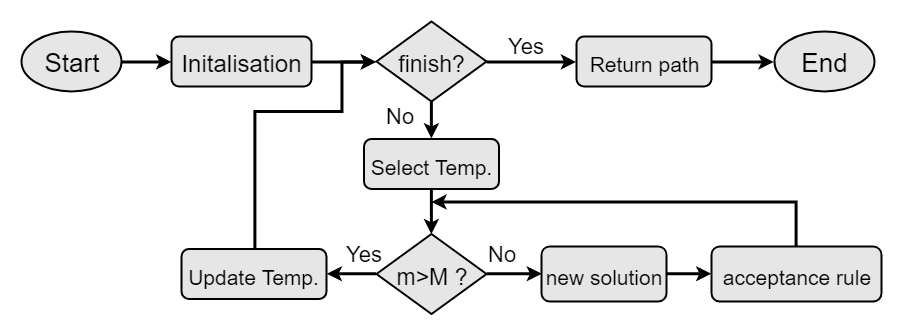
\includegraphics[width=\textwidth]{Figures/system_implementation/LBSA.png}
  \caption{Block diagram of the Simmulated Annealing metaheuristic.}
  \label{fig:LBSA}  
\end{figure}